\documentclass[12pt,a4paper,twoside,openright]{book}

%%%%%%%%%%%%%%%%%%%%%%%%%%%%%%%%%%%%%%%%%%%%%%%%%%%%%%%%%%%%%%%%%%%%
%  Template per Tesi di Laurea                                     %
%                                                                  %
%%%%%%%%%%%%%%%%%%%%%%%%%%%%%%%%%%%%%%%%%%%%%%%%%%%%%%%%%%%%%%%%%%%%

               %%%%%%%%%%%%%%%%%%%%%%%%%%%%%%%%%%%%%%
               %    Scelta dei package da usare     %
               %%%%%%%%%%%%%%%%%%%%%%%%%%%%%%%%%%%%%%


\usepackage[dvips]{graphicx}
\usepackage{graphics}
\usepackage[normalem]{ulem}
\usepackage[utf8]{inputenc}
\usepackage[italian,finnish,british]{babel}
\usepackage{float}
\usepackage{graphicx,algorithm,algorithmic}
\usepackage{amsmath,amsfonts,amssymb,amsthm}
\usepackage{epsfig}
\usepackage{deistesi}
\usepackage{fancyhdr}
\usepackage{xspace}
\usepackage[colorlinks=false]{hyperref}
\usepackage[avantgarde]{quotchap}
\renewcommand\chapterheadstartvskip{\vspace*{-5\baselineskip}}
\renewcommand\sectfont{\sffamily\bfseries}
\usepackage{mathptmx}       % selects Times Roman as basic font
\usepackage{helvet}         % selects Helvetica as sans-serif font
\usepackage{courier}        % selects Courier as typewriter font
\usepackage{type1cm}        % activate if the above 3 fonts are
\usepackage{makeidx}         % allows index generation
\usepackage{multicol}        % used for the two-column index
\usepackage[bottom]{footmisc}% places footnotes at page bottom
\usepackage{times}
\usepackage{subfigure}
\usepackage{stmaryrd,mathtools}
\usepackage{cleveref}


\newcommand{\bnfs}[0]{\;|\;}
\newcommand{\opar}[0]{\;|\;}
\newcommand{\sq}[0]{\oplus}
\newcommand{\tuple}[2]{#1\langle #2\rangle}
\newcommand{\tupled}[2]{#1[#2]^{\Rightarrow}}
\newcommand{\actrate}[2]{#1^{#2}}
\newcommand{\leave}{{}}
\newcommand{\near}[3]{#1\!\stackrel{#3}{\rightsquigarrow}\!#2 }
\newcommand{\scope}[2]{\llbracket #1 \rrbracket_{#2}}
\newcommand{\law}[1]{[#1]}
\newcommand{\firing}[3]{#1^\rightsquigarrow(#2,#3)}
\newcommand{\shfiring}[1]{#1^\rightsquigarrow}

\newcommand{\defn}[2]{\mathit{def} #1 := #2}
\newcommand{\defnarr}[2]{\mathit{def} #1 & := & #2}
\newcommand{\call}[1]{call\, #1}


               %%%%%%%%%%%%%%%%%%%%%%%%%%%%%%%%%%%%%%
               %  Scelta del tipo di font da usare  %
               %%%%%%%%%%%%%%%%%%%%%%%%%%%%%%%%%%%%%%

%\usepackage{times,mathptm}
%\usepackage{palatino,mathpple}
%\usepackage{bookman}
%\usepackage{newcent}

               %%%%%%%%%%%%%%%%%%%%%%%%%%%%%%%%%%%%%%%%
               % Scelta delle dimensioni della pagina %
               %%%%%%%%%%%%%%%%%%%%%%%%%%%%%%%%%%%%%%%%

\setlength{\textwidth}{16.0cm}
\setlength{\textheight}{21cm}
\setlength{\footskip}{3cm}



               %%%%%%%%%%%%%%%%%%%%%%%%%%%%%%%%%%%%%%
               %  Informazioni generali sulla Tesi  %
               %    da usare nell'intestazione      %
               %%%%%%%%%%%%%%%%%%%%%%%%%%%%%%%%%%%%%%

\titolo{Engineering complex computational ecosystems}
\candidato{Danilo Pianini}
\annoaccademico{2015}
\facolta{Ingegneria}
\dipartimento{DEIS - Dipartimento di Elettronica, Informatica e Sistemistica}
\dottorato{PhD Course in Electronics, Computer Science and Telecommunications}
\settoreconcorsuale{09/H1}
\settoredisciplinare{ING-INF/05}
\ciclo{XXVII}
\tutor{Antonio Natali}
\relatore{Mirko Viroli}
% \correlatoreb{Andrea Roli}
% \correlatorec{Mirko Viroli}
\coordinatore{Alessandro Vanelli Coralli}
\dedica{
\emph{\mbox{~~~~~~~~~~~~~~~~~~~~~~~~~~~~~~~~~~~~~~~}Lorem ipsum dolor sit amet. \\
%
\mbox{~~~~~~~~~~~~~~~~~~~~~~~~~~~~~~~~~~~~~~~~~~~~}consectetur adipiscing elit.\\
%
\mbox{~~~~~~~~~~~~~~~~~~~~~~~~~~~~~~~~~~~~~~~~~~~~}Sed fringilla quis mauris id sagittis everything.}\\ \\ \\ \\
\noindent \emph{\textbf{Acknowledgements}}\\ \\
Curabitur commodo dictum risus laoreet tincidunt. Sed dapibus nec ex sit amet consequat. Quisque cursus est sit amet lectus tempor, nec egestas sapien rutrum. Sed dapibus consequat egestas. Quisque blandit, tellus et molestie interdum, augue est molestie lorem, tristique congue metus massa sed eros. Vivamus fermentum erat a faucibus porta. Praesent sit amet risus leo. Integer venenatis lectus sed euismod euismod. Ut pulvinar fermentum sagittis. Aliquam maximus nisl velit, ac varius tellus dignissim in. Fusce nibh dolor, blandit vel nisl non, vehicula tincidunt lorem. Suspendisse fringilla magna ac justo fermentum, nec accumsan odio sollicitudin. Maecenas consectetur, nulla sit amet ultricies pretium, metus sapien posuere turpis, in lobortis tellus turpis ac ipsum. Aliquam sollicitudin augue a aliquam volutpat. Mauris bibendum nunc id est ullamcorper, nec feugiat elit dapibus.\\
%
Duis tincidunt maximus justo, id convallis mauris mattis congue. Maecenas ullamcorper laoreet lacinia. Praesent luctus dictum metus, sed ultrices dui. Fusce fringilla eu est sit amet porta. Aliquam ornare eleifend congue. Aliquam orci urna, accumsan nec metus a, tincidunt pulvinar augue. Nunc eu vulputate lectus. Morbi placerat varius purus at scelerisque. Mauris malesuada ut massa non porta. Quisque ac efficitur odio. Aliquam scelerisque dapibus felis in ullamcorper. Pellentesque ullamcorper massa quis nibh suscipit elementum. Suspendisse tincidunt, sem non porta consectetur, arcu mauris mollis mi, ut commodo libero diam ut risus.
}
\data{March 2015}
\signature{\emph{Danilo Pianini}}

              %%%%%%%%%%%%%%%%%%%%%%%%%%%%%%%%%%%%%%
               % Fine Preambolo                     %
               % Inizio tesi                        %
               %%%%%%%%%%%%%%%%%%%%%%%%%%%%%%%%%%%%%%

\begin{document}

%%%%%%%%%%%%%%%%%%%%%%%%%
% inizio prefazione
%
% pagina del titolo, indice, sommario
%%%%%%%%%%%%%%%%%%%%%%%%%
\frontmatter
\maketitle
\pagestyle{plain}
\tableofcontents

\chapter*{\centering Abstract}
\addcontentsline{toc}{chapter}{Abstract}

This work presents advancements of the latest three years in the engineering techniques for self-organising pervasive ecosystems of devices and services.
%
The inherent complexity of such systems poses new challenges to those who try to dominate the complexity by applying the principles of engineering.

The recent growth in number and distribution of devices with decent computational and communicational abilities, that got suddenly accelerated with the massive diffusion of smartphones and tablets, is envisioning a world with a much higher density of devices in space.
%
This already high device density is probably going to consistently rise if the diffusion of wearable devices gets momentum.
%
Also, communication technologies seem to be focussing on short-range device-to-device (P2P) interactions, with technologies such as \btle{} and Near-Field Communication getting more and more diffused.

Locality and situatedness become key to provide the best possible experience to users, and the classic model of a centralised, enormously powerful server gathering data and processing it is likely to get less and less efficient with device density.
%
Accomplishing complex global tasks without a centralised controller responsible of aggregating data from devices, however, still is a challenging task.
%
In particular, it is hard to understand which device-local programs could properly interact and guarantee a certain global service level.
%
Such local-to-global issue makes the application of engineering principles challenging at least.

In this work, I lay the foundations of my contribution by first analysing the state of the art in coordination systems, namely in those software frameworks devoted to control and promote interactions among independent software entities.
%
I then motivate my work, by describing the main issues of pre-existing tools and practices and identifying the improvements that would benefit the design of such complex software ecosystems.
%
My contribution is described in \Cref{contribution}, and can be divided in three main branches: i) a novel simulation tool for pervasive ecosystems, ii) introduction of novel and improvements over existing self-organisation patterns, iii) the creation of a new language and interpreter based on ``field calculus'' and its integration with the previously mentioned simulator.
%
Finally, I draw conclusions and future works.

\mainmatter

% stile della pagina
\pagestyle{fancy}
\fancyhead[LE,RO]{\bfseries\thepage}

\part{Background}
\label{background}
\chapter{Pervasive devices}
\label{pervasive-devices}

It is no mystery that, with the huge progresses of miniaturisation, computational-capable devices are populating the world.
%
The diffusion got momentum with affordable ``personal computers'' that made their way in a one-device-per-family world.
%
Laptops boosted the process, offering user a personal and mobile device.

The pervasive revolution, however took place when the phones became ``smart'', and with the subsequent improvements in the communication technologies.
%
In this chapter, I try to briefly walk the path of success of personal mobile devices, describing also the probable newcomer, namely the wearable devices.
%
I also focus on the current status of the communication protocols, their range and usage, and I try to foresee which world are we going to build if the current trend continues.

\section{Smart, portable devices}

\begin{figure}
	\centering
	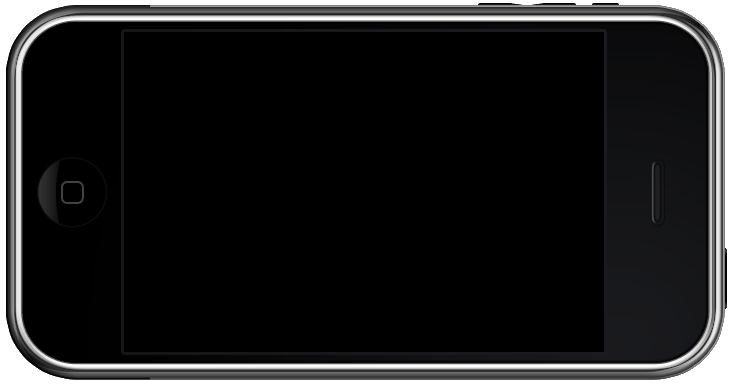
\includegraphics[width=0.99\textwidth]{img/iphone}
	\caption{Apple iPhone is one of the first devices without any physical keyboard, and the first smartphone to gain worldwide success. \emph{Source: Wikimedia.}}
	\label{img:iphone}
\end{figure}

When Apple in 2007 released the first iPhone (\Cref{img:iphone}), a mobile revolution started.
%
Even though other manufacturers proposed products similar to iPhone under the point of view of communication technologies and computational capabilities in the same time frame (e.g. Nokia N810), the Apple's smartphone was the first gaining widespread adoption.
%
It is not really relevant for this work to understand if the branding, the design, the multi-touch finger based interaction UI or the feature set was the key of its commercial success: what really matters is that, starting 2007, every person began to carry with her a personal device featuring both the abilities to communicate and compute.
%
The reason, besides the success of iPhone in the higher segment of the phone market, is mainly to attribute to the widespread diffusion of similar but cheaper and less powerful devices in the lower segments.
%
This kind of devices ultimately pushed the market share of the dominating today's mobile operating system, Google's Android.

This trend towards a higher diffusion got another leap forward three years later, in 2010, when a device with a feature set similar to iPhone, but with no phone abilities  and a bigger screen was released: the iPad.
%
As iPhone gave new vitality and perspectives to the phone arena, iPad revitalised a market that was languishing: the tablets.
%
Tablet devices as they were conceived before iPad launched were nothing more than small laptops with a screen that could be rotated or detached from the keyboard, and a touch-screen normally used with the help of a pen.
%
They changed from devices designed for a professional niche to widespread tools, up to the point that Gartner forecasts their shipments to overtake in 2015 those of desktop PC and laptops aggregated \footnote{\url{http://www.gartner.com/newsroom/id/2791017}}.

The new frontier of pervasive is probably the wearable technology. Smartphones were precursors, they substituted mobile phones introducing new features and they have potential to substitute our wallets (see, for instance, payments through NFC technology) and keys, becoming the only object we need to carry with us in our pockets.
%
Still there are other accessories which are hard to replace, above all watches and glasses.
%
Yes, smartphone can easily show the current time accurately (and, to be honest, also feature phones had this feature well before 2007), but they require the user to pick them from the pocket, turn them on, and sometimes, depending on privacy settings, also unlock them.
%
The whole operation, takes a much longer time and higher effort with respect to just rotating a wrist.
%
This might be the reason why, despite the explosive expansion of smartphones, the wristwatches market did not declined, as an analysis from MarketWatch points out \footnote{\url{http://www.marketwatch.com/story/the-watchs-time-isnt-up-2013-07-01}}.

\begin{figure}
	\centering
	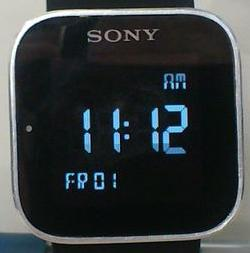
\includegraphics[height=5cm]{img/sony-sw}
	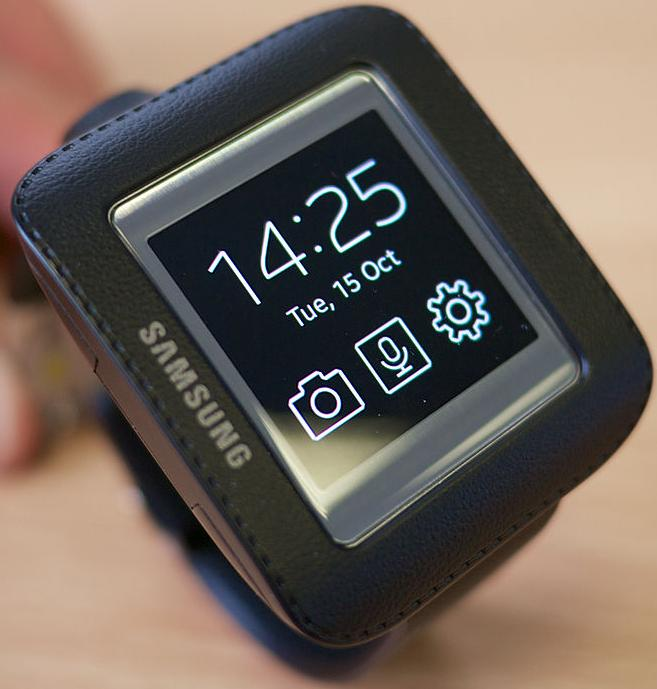
\includegraphics[height=5cm]{img/samsung-gg}
	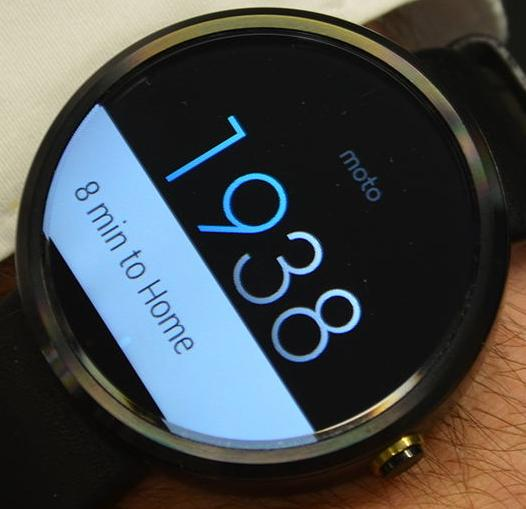
\includegraphics[height=5cm]{img/moto360}
	\caption{Smart watches. From left to right: Sony Smartwatch \emph{(Source: Alex S.H. Lin)}, Samsung Galaxy Gear \emph{(Source: Karlis Dambrans)}, Motorola Moto 360.}
	\label{img:watches}
\end{figure}

There is room for manufacturers to create new portable devices.
%
Sony, starting 2012, has produced a series of smartwatches, such as those in \Cref{img:watches} that pair with a smartphone and provide quick access to some of its functionalities.
%
The success of such solution is not huge, but despite that many other companies are interested in this market: Samsung, Motorola and Apple presented devices meant to replace the classic wristwatch, a clear sign that this market is in expansion.
%
At the time of writing, the main issues that slow the widespread adoption of such solutions are battery duration and dependence on a smartphone.

\begin{figure}
	\centering
	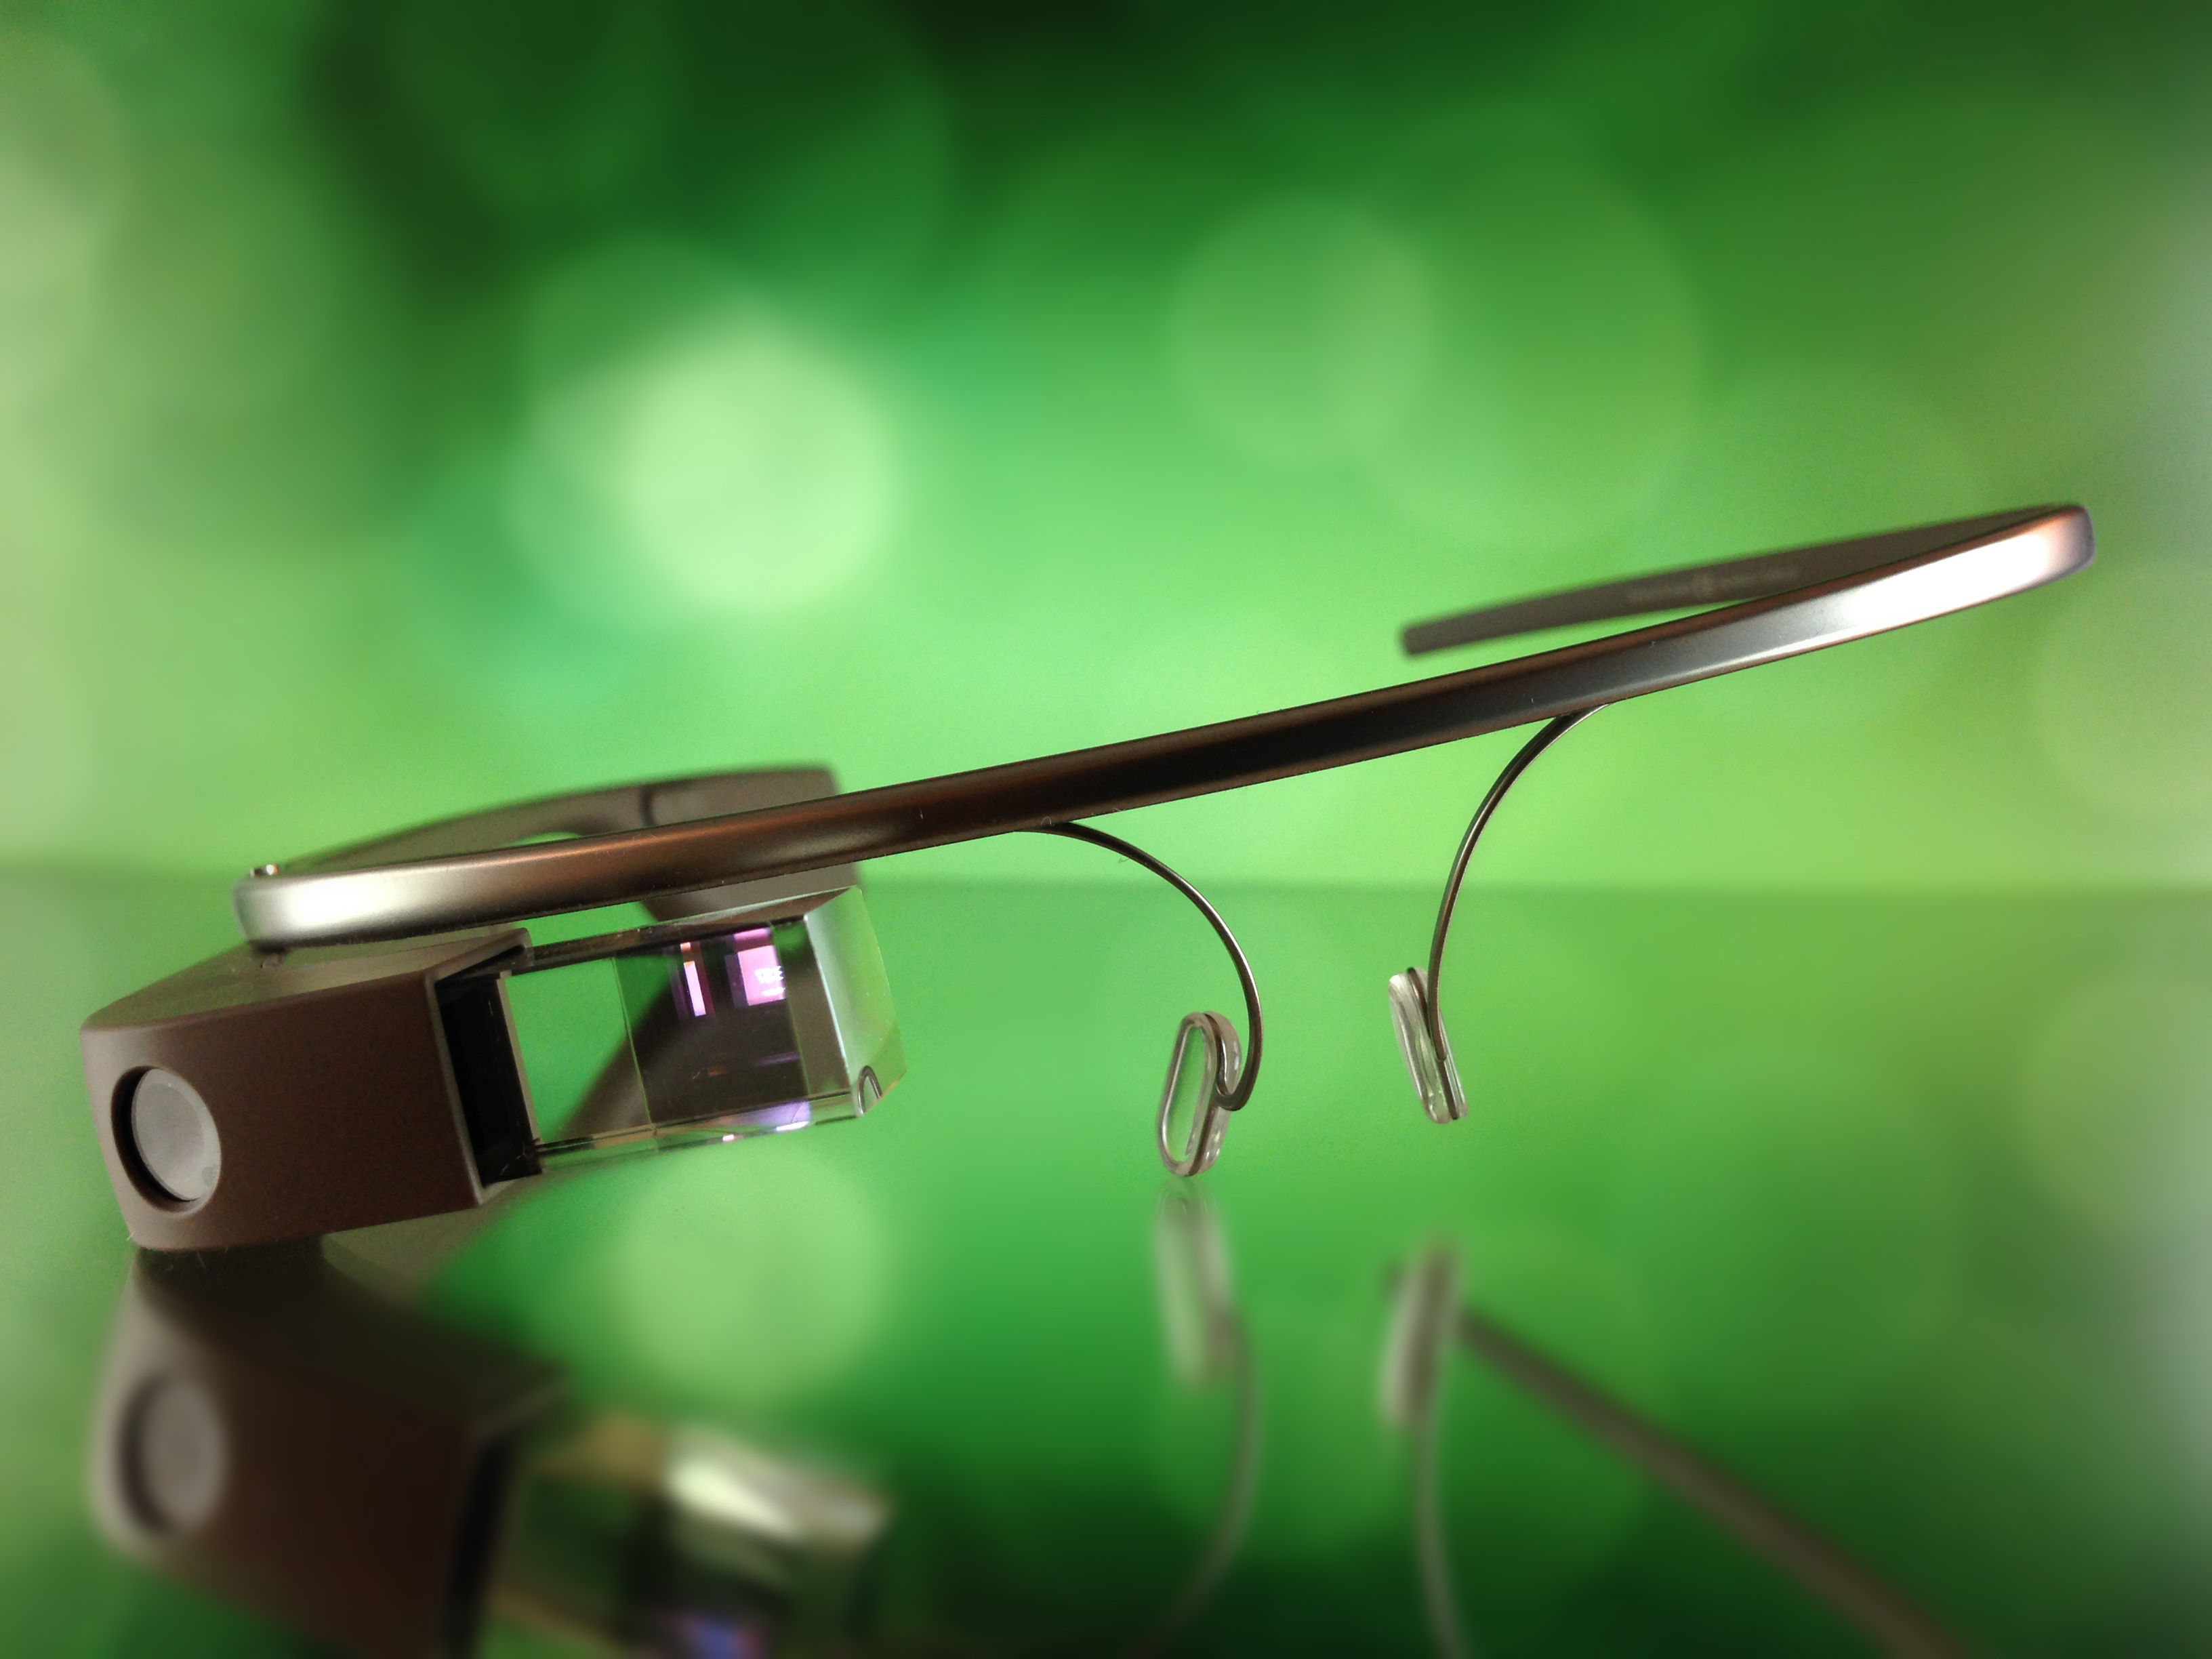
\includegraphics[width=0.99\textwidth]{img/gglass}
	\caption{Google Glass. In this image, it is possible to see both the camera (on the left hand side) and the semi-transparent head-mounted display. Are those devices going to be part of our everyday life? \emph{Source: Wikimedia.}}
	\label{img:gglass}
\end{figure}

Another notable attempt to make a common accessory smarter is Google Glass project, depicted in \Cref{img:gglass}.
%
Their goal is to enhance the experience of wearing glasses by attaching a device with a camera, an optical head-mounted display, and the abilities to locate itself and communicate with other devices.
%
Google Glass, at the time of writing, are way to expensive (with the kit sold at \$1500) for being able to penetrate the general public, but they are an interesting anticipation of possible future devices.

On the same line of such wearable devices, a discrete success is being achieved by the so called ``fit bands''.
%
They are bracelets equipped with low energy sensors, mainly accelerometers and gyroscopes, which are used to keep track of user's activity.
%
Depending on the model, they can be used to monitor some user's health parameters, such as the number of steps walked per day or heartbeats.
%
They normally work along with another device, a smartphone or a tablet.
%
Such devices, due to their precise market niche and reasonably low price (the Chinese manufacturer Xiaomi recently introduced a low-end wristband at around \$15) are having a notable success.

The wearable devices segment also includes less common devices such as ``smart shoes'' and materials that can be used to make clothing, such as e-textiles.
%
It is a market in expansion, greatly beneficing from recent increases in performance per watt efficiency.
%
If the trend continues, it is likely that we will more and more powerful wearable devices on sale at cheaper and cheaper prices, and a consequent widespread diffusion.
%
The same sort may occur to other parts of our life: kitchen gear, indoor lights and many other objects are getting more and more ``smart'' around us.
%
We may, literally, end up with a world where every single object embeds computational and communicational abilities.

A problem arise: how can software engineers deal with such a complexity?

\section{Communication technologies}

Besides miniaturisation, and as a consequence the increase of computational density in space, another factor played a fundamental role in the world of pervasive computing: the ability to communicate, and in particular the ability to rely on wireless communication, which is of paramount importance when considering mobility.

In later years, many communication means arose.
%
They largely differ in terms of range, protocols, and availability.
%
In this section, I try to resume the most diffused technologies available on today's devices, but the reader is warned: keep in mind that such technologies are evolving very quickly, and the scenario is incredibly fluid.

\subsection{International Mobile Telecommunications}

This first mean of communication is designed to allow mobile devices to access the Internet from anywhere in the world, relying on the existing mobile phone infrastructure.
%
Such technologies are meant to be used with the standard IP protocols, and they are normally used to get access to public services, in particular to the world wide web.
%
They are not designed for a local peer-to-peer (P2P) communication, and as a consequence they provide no mean to exploit locality.
%
The diffusion of such communication protocols is widespread, in particular among smartphones.
%
Due to the fact that they rely on the mobile phone network, they require a contract with a mobile telecommunications provider, and as such they are much less diffused in tablets and other portable devices.

\begin{figure}
	\centering
	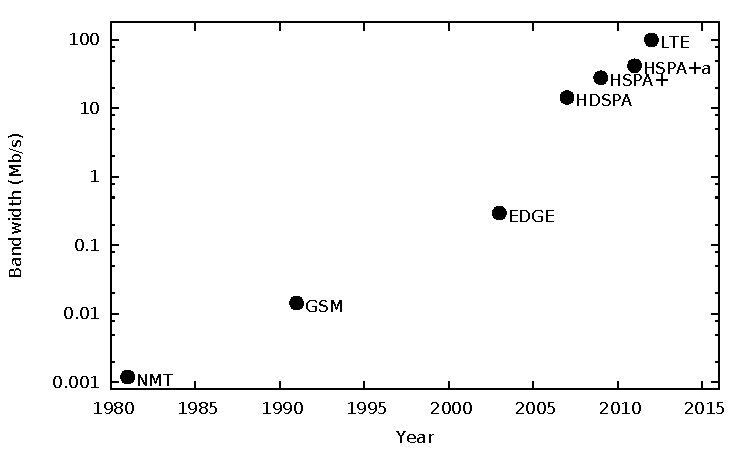
\includegraphics[width=0.99\textwidth]{img/charts/mobile-data-performance}
	\caption{
		Maximum download bandwidth available for mobile devices with time.
		%
		Each point is labelled with the specific communication technology name.
		%
		For the most recent multiple-input-multiple-output (MIMO) technologies, such as LTE, a conservative single input channel was used.
	}
	\label{img:mobile-bandwidth}
\end{figure}

The possibility of accessing the Internet from everywhere is probably one of the key bricks that allowed for the huge success of smartphones in today's world.
%
As \Cref{img:mobile-bandwidth} shows, the bandwidth available grew exponentially with time, to the point that in some countries (e.g. in Italy, at the time of writing) the best available mobile connections offer a higher performance than the best available home connection
%
\footnote{At the time of writing, Telecom Italia Mobile offers mobile connections on LTE with a download bandwidth up to 225Mb/s.
%
Fastweb, the company offering the faster solutions for fiber-to-home connections, goes up to 100Mb/s.}.
%
Such performance unlock the possibility of fully exploiting the possibilities of the world wide web, including cloud services and fruition of multimedia content.

If bandwidth is not currently an issue for international mobile telecommunications, the situation is well different when it comes to device density.
%
Any of us probably experienced network availability issues when participating crowded events, such as concerts or sport events.
%
The current technology, in fact, makes all the network user share the same physical resources: when the device density is too high, there is simply not enough space in the frequency spectrum to grant a decent bandwidth to everyone.
%
Future networks (5G, and presumably those that will follow) are focussing toward this issue among others \cite{5g}.
%
In particular, a so-called ``spectrum crunch'' is expected due to the expected traffic increase (thousand fold over this decade and still growing into the next), that could not be faced simply with the foreseen steady increase of the spectrum allocated for mobile communication, and will require technological advances \cite{spectrum-crunch}.

\subsection{WiFi}

WiFi technology is the most diffused technology for wireless local networking.
%
It is widely diffused, integrated in all smartphones and tablets and also in other devices, such as printers and TVs.

\subsection{Bluetooth}
\subsection{NFC}

\section{Towards a P2P world?}
Despite the ongoing research on 5g, we want higher density. Privacy as issue, locality.

IPv6, locality, density

\chapter{Coordination infrastructures}
\label{coordination-infrastructures}
\section{The issue of coordination}
why do we want a middleware
\section{Nature inspiration}
see what exists, mimic
\section{Coordination platforms and languages}
what is there already
\subsection{Linda}
and swarmlinda
\subsection{TOTA}
\subsection{TuCSoN}
and the semantic extension
\subsection{Biochemical tuple spaces}
and MoK?
\subsection{SAPERE}
general idea of sapere, grounds on previous works.
\subsection{Proto and Field Calculus}
\subsubsection{Alignment}
\section{Spatial patterns}
what is a pattern
patterns before sapere (gossip, gradient)
problems with gradient
\section{Engineering and tools}
methodological issues, deployment and testing issues, need of simulation
\subsection{General purpose frameworks}
Repast, netlogo
\subsection{Specific simulators}
network simulators (the one, ns2)
biological simulators (ask Sara)

Specific per-use simulators, gener

\part{Motivation}
\chapter{Shortcomings of coordination infrastructures}
\section{Engineering emergence}
\section{Local to global}
\chapter{Shortcomings of existing tools}
\section{Specific tools: expressiveness}
\section{General purpose tools: performance}

\part{Contribution}
\label{contribution}
\chapter{Integrated tools for designing pervasive ecosystems}
\section{Chemical inspired MABS}
\section{Meta-meta model}
\section{Chemical meta-model}
\subsection{Simulation of a morphogenesis model}
\section{SAPERE meta-model}
\section{Advanced features}
\subsection{Distributed statistical analysis}
\subsection{Real world maps}

\chapter{Self-organisation patterns}
SAPERE
\section{Crowd evacuation}
\section{Self composition}
\section{Semantic resource discovery}
\section{Anticipative adaptation}
\section{Crowd disasters prediction}
\section{HPC at the urban scale}

\chapter{Aggregate programming languages}
Protelis
\section{Higher order functions in field calculus}
\subsection{Impact on alignment}
\section{Java integration}
\section{Alchemist as a simulation platform}
\section{Alchemist as a core engine for real devices}

\part{Conclusion}
\chapter{Results achieved}

\chapter{Future and ongoing work}
\section{Biochemical meta model for Alchemist}
ciao

%\appendix
%\input{appendix-a.tex}
%\input{appendix-b.tex}
%\input{appendix-c.tex}

%\input{publication.tex}

\part{Bibliography}

%===============================================================================
\small\protect\newpage\addcontentsline{toc}{chapter}{Bibliography}
\bibliography{thesis}
\bibliographystyle{alpha}
%===============================================================================

%\listoffigures
%\listoftables

\end{document}
